\section{PyExaFMM}

\subsection{Motivation}
\begin{frame}{Motivation}
    \begin{itemize}
        \item Python has emerged as a standard in scientific and data intensive computing
        \item Desire a high quality software implementation which is also highly performant and easily portable
        \item Tradeoff performance of compiled languages for engineering ease, and portability
    \end{itemize}
\end{frame}

\subsection{Goals}
\begin{frame}{Goals}
    \begin{itemize}
        \item Create a performant 3D Python implementation of the KIFMM
        \item Write software in an extensible and well tested way
        \item Take advantage of distributed and parallel computing concepts as much as possible
    \end{itemize}
\end{frame}

\subsection{Outcomes}
\begin{frame}{Outcomes - Vectorised Data Structures}
    \begin{figure}
        \centering
        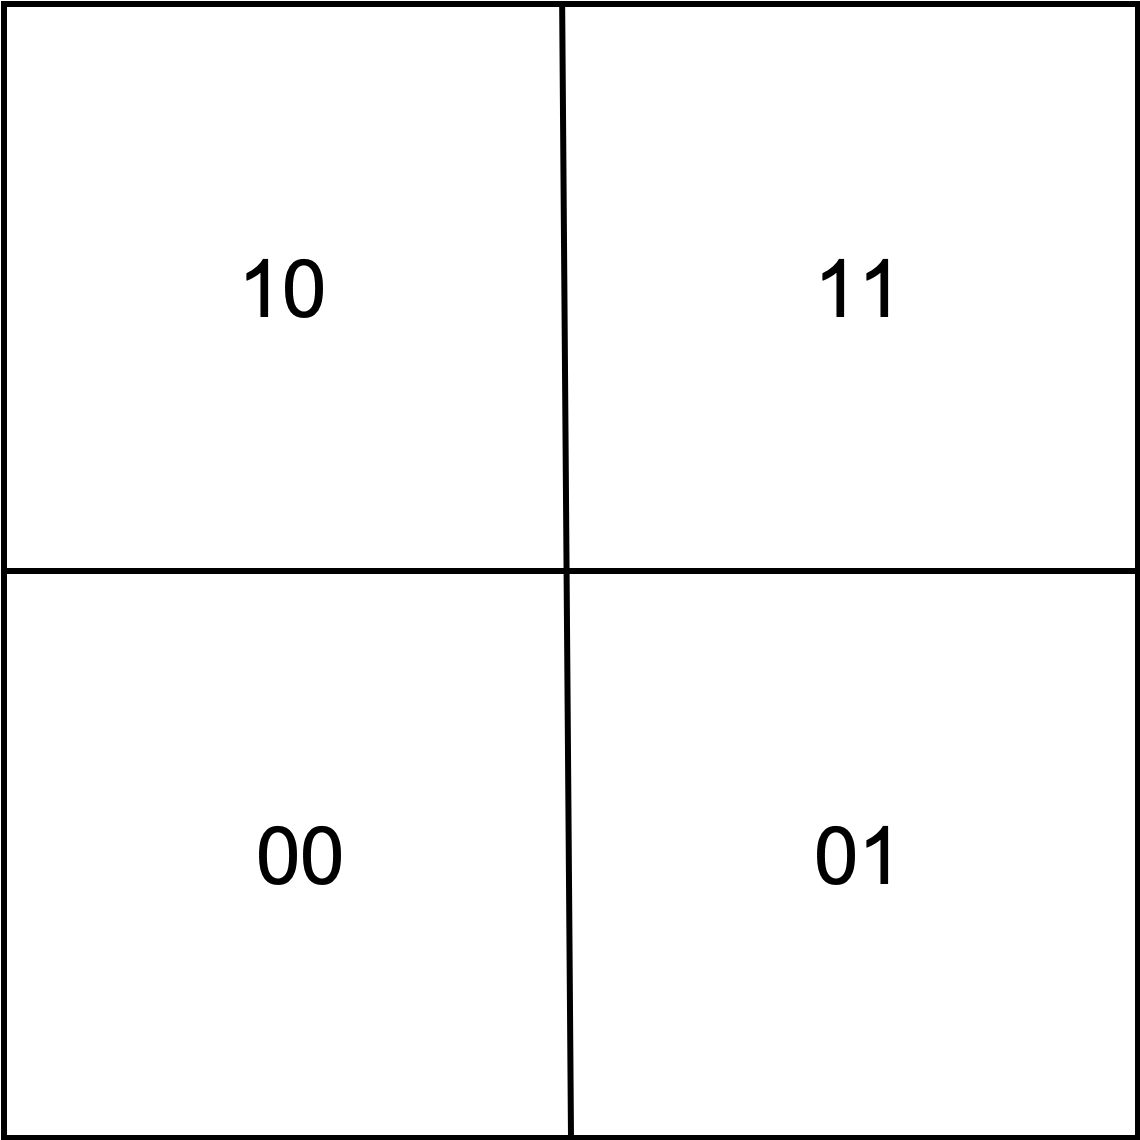
\includegraphics[width=0.5\textwidth]{assets/morton_coarser.png}
    \end{figure}
    \vspace{50pt}
\end{frame}

\begin{frame}{Outcomes - Vectorised Data Structures}
    \begin{figure}
        \centering
        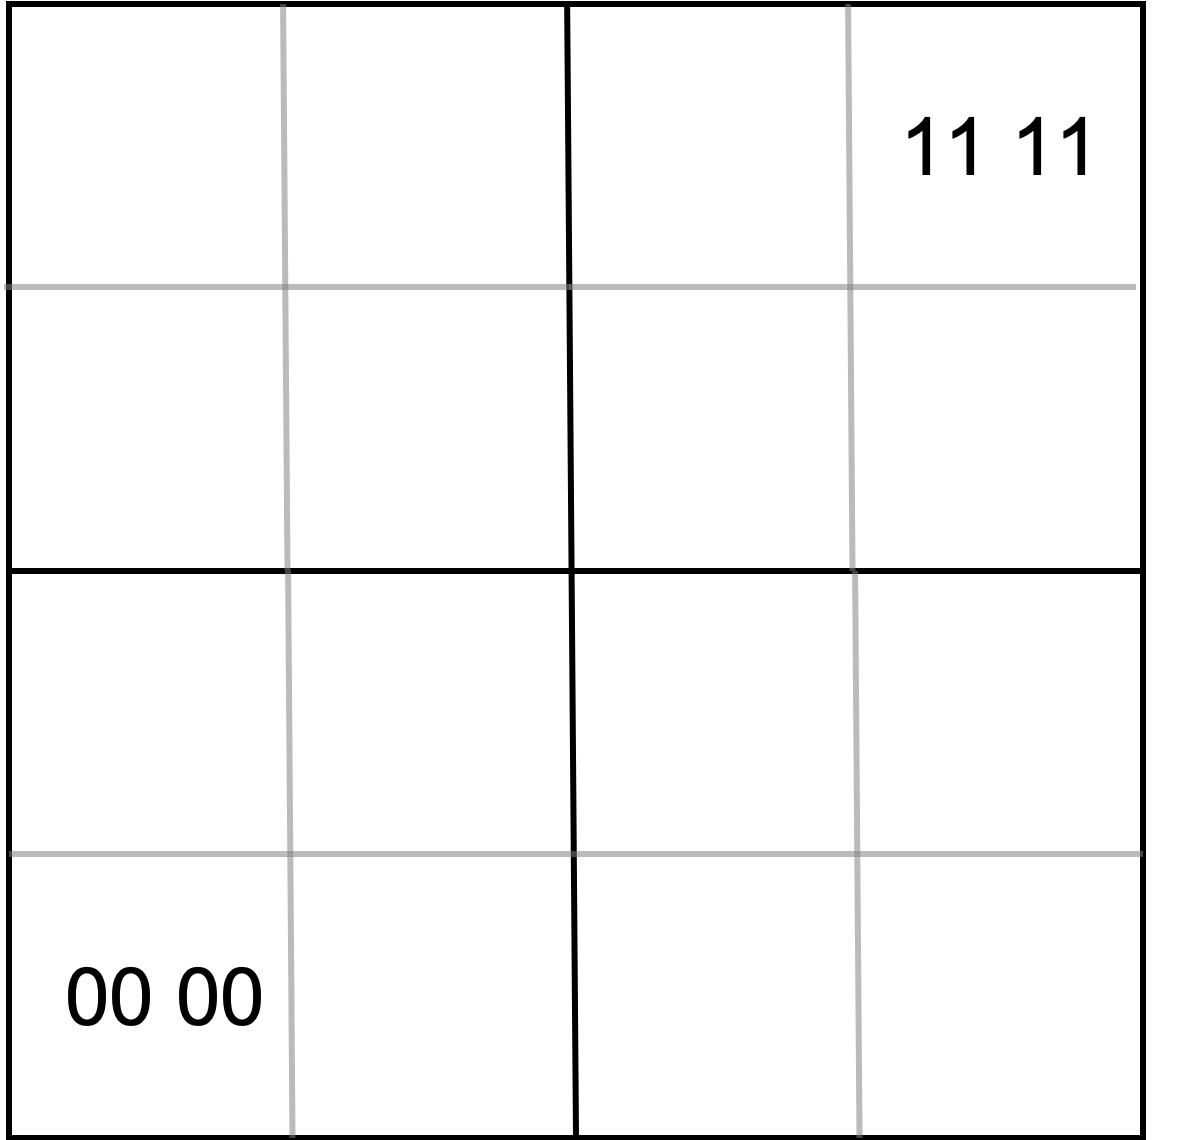
\includegraphics[width=0.5\textwidth]{assets/morton_finer.png}
    \end{figure}
    \vspace{50pt}
\end{frame}

\begin{frame}{Outcomes - Vectorised Data Structures}
    \begin{figure}
        \centering
        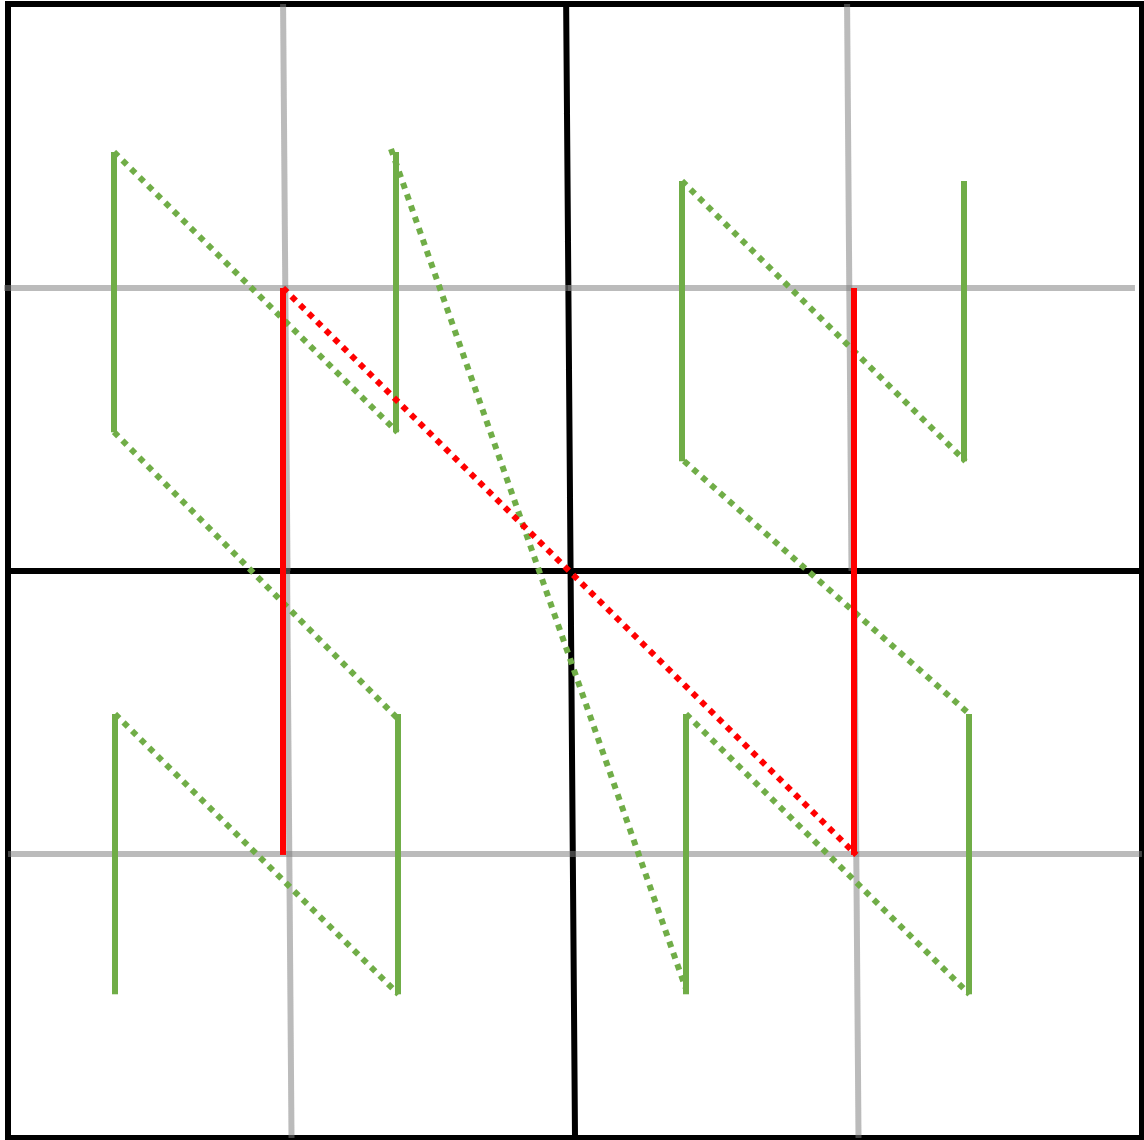
\includegraphics[width=0.5\textwidth]{assets/morton_2d.png}
    \end{figure}
    \vspace{50pt}
\end{frame}

\begin{frame}{Outcomes - Vectorised Data Structures}
    \begin{figure}
        \centering
        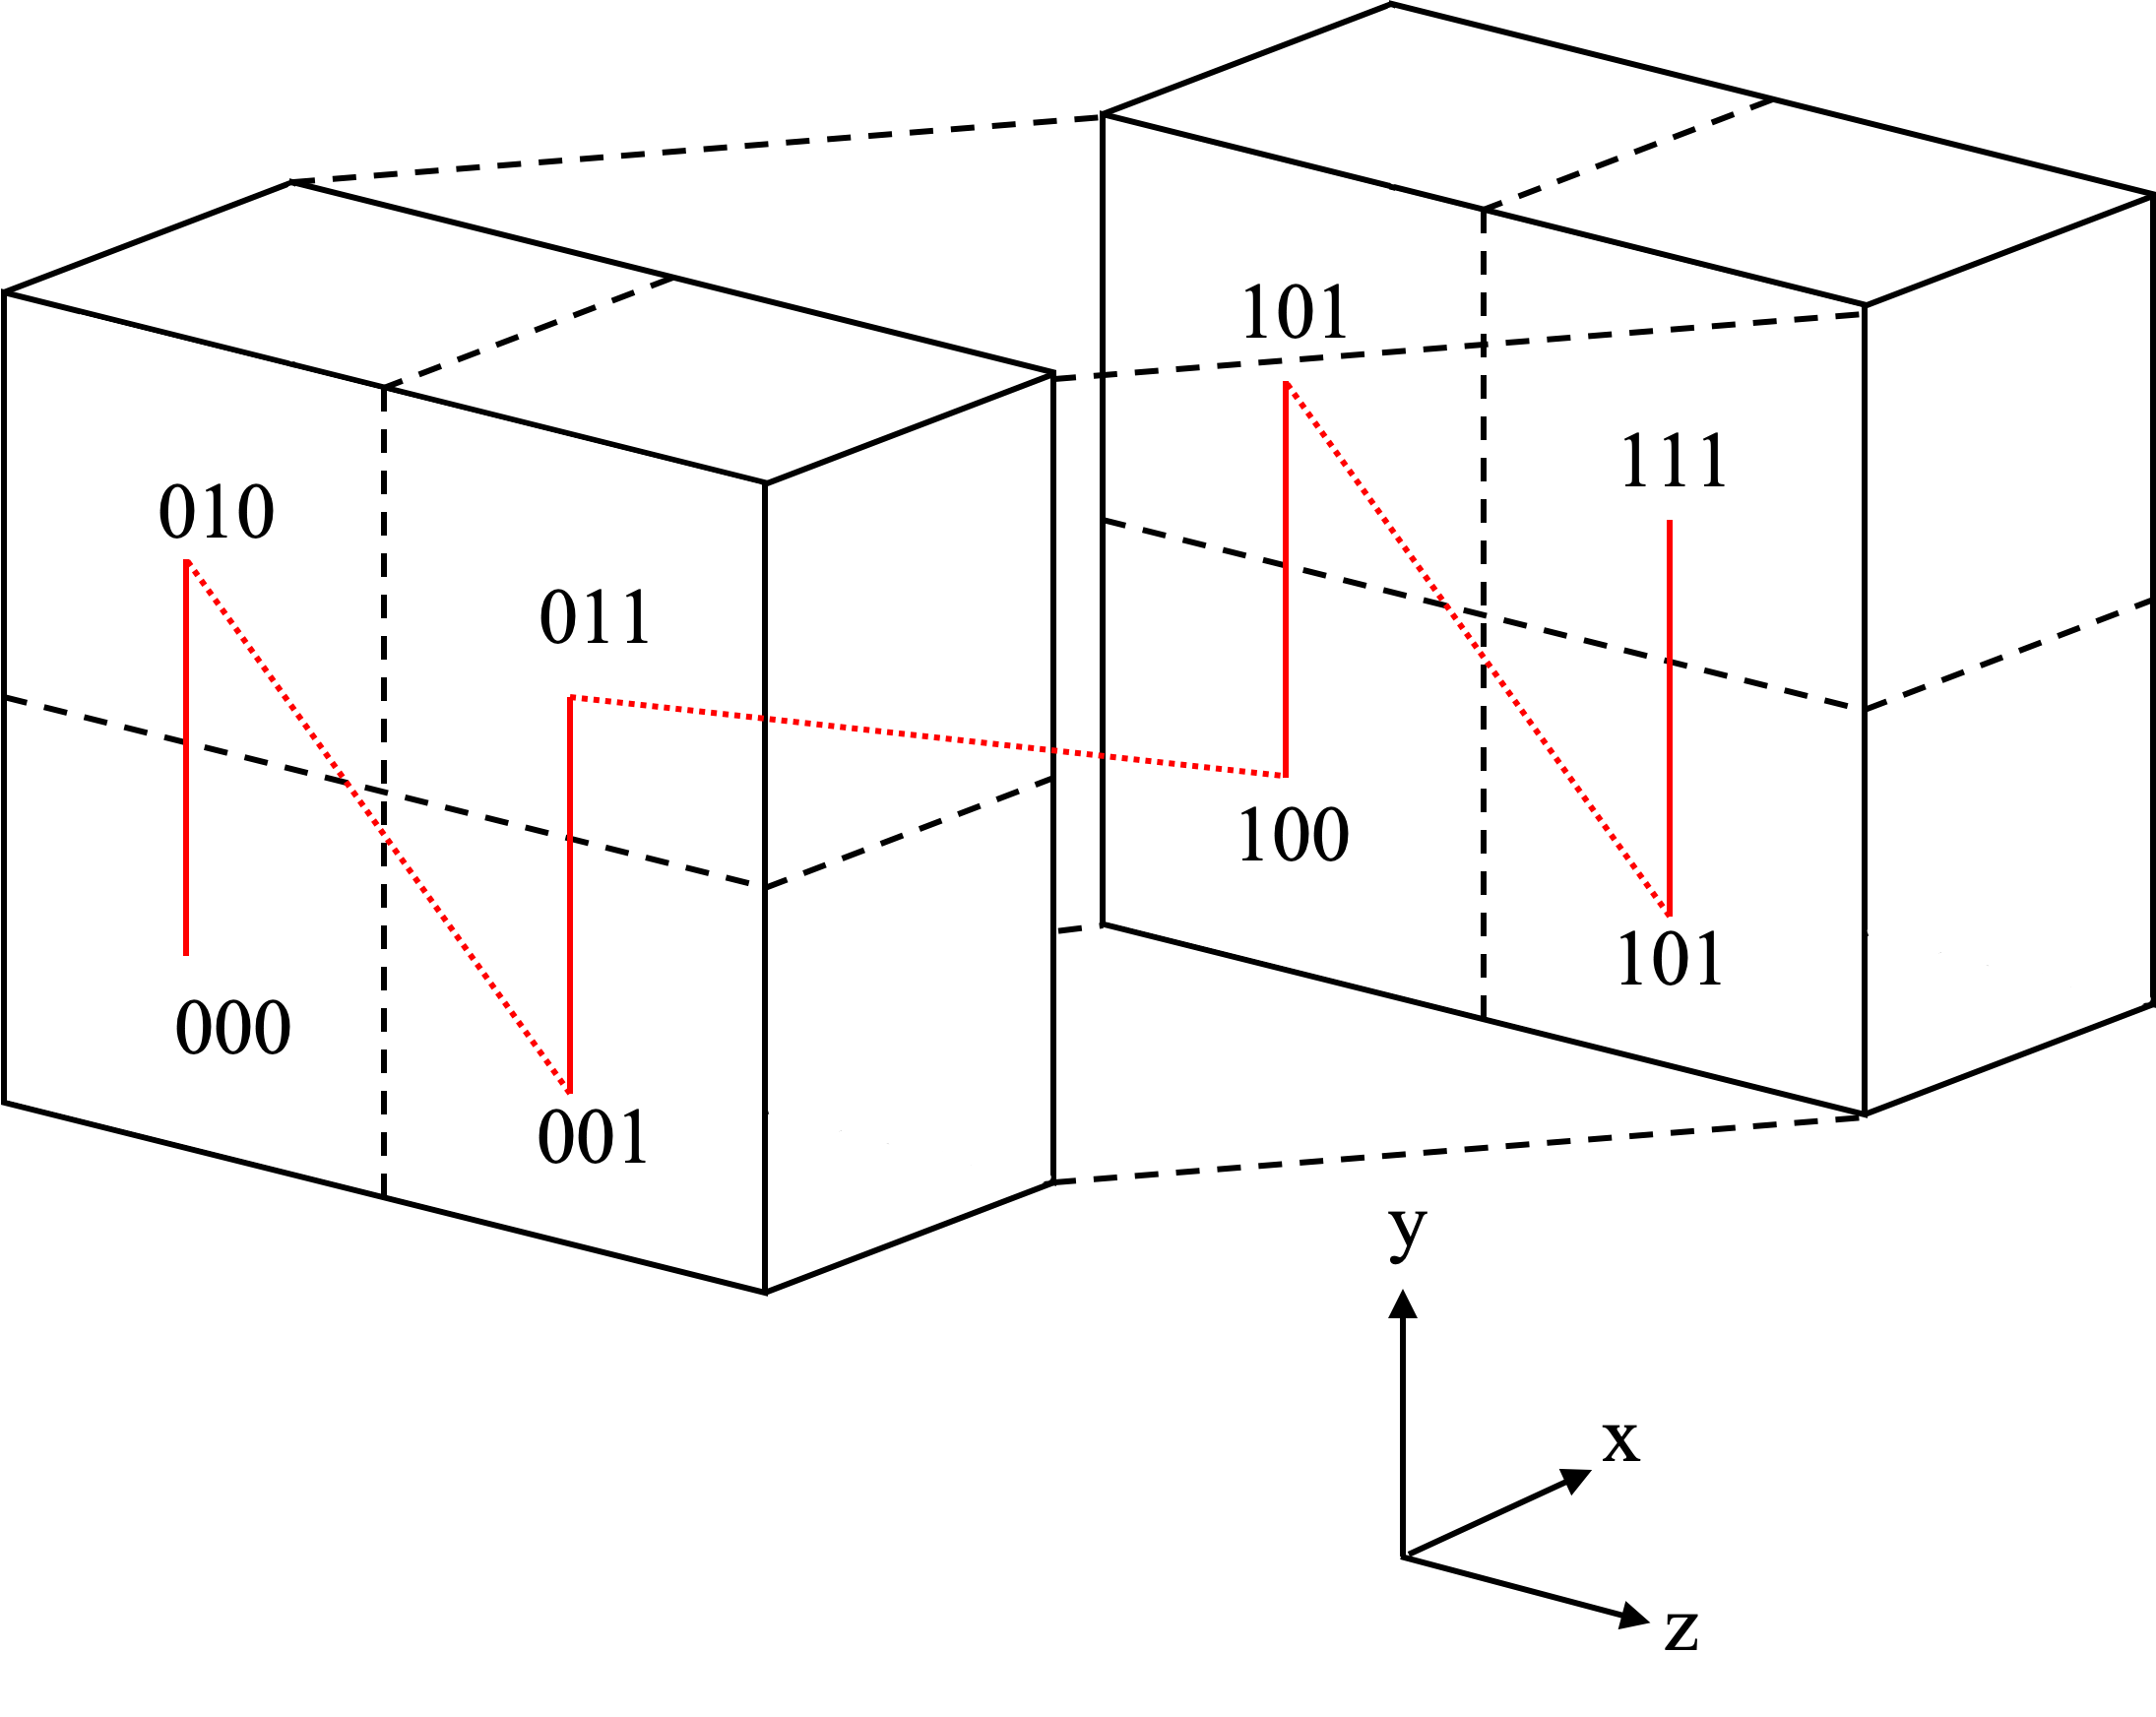
\includegraphics[width=0.6\textwidth]{assets/morton_3d.png}
    \end{figure}
\end{frame}

\begin{frame}{Outcomes - JIT Compilation}
    \begin{itemize}
        \item Pre-analyse interpreted bytecode for reused calculations, compile into assembly and cache
        \item Use Numba on top of Numpy Containers
    \end{itemize}
\end{frame}

\begin{frame}{Outcomes - Multiprocessing \& Operator caching}
    \begin{itemize}
        \item Pre-compute and cache all operators, used in rhs of least squares problem, ($\phi^A = (\alpha I + K_A^*K_A)^{-1}K_B\phi^B$)
        \item Use process level parallelism to distribute the computation
        \item Use HDF5 for rapid loading to memory in comparison to simple serialisation
    \end{itemize}
\end{frame}

\begin{frame}{Outcomes - Low-Rank SVD Compression}

    \begin{itemize}
        \item $I$ - number of source boxes in interaction list of a given target box
    \end{itemize}

    \begin{flalign}
        K_{\text{source}} &=  (\alpha I +  K_{\text{source}}^* K_{\text{source}})^{-1}K_{\text{target}}\\
        K_{\text{concatenated}} &= \left [ K_1 | K_2 | ... | K_I \right] \> \> \text{   ,  where,  } \{K_i | i \in [1, 2, ..., I]\}
    \end{flalign}
\end{frame}


\begin{frame}{Outcomes - Low-Rank SVD Compression}
    \begin{itemize}
        \item The rank of the full concatenated matrix is $r$
        \item Can truncate sum to target rank, $k$, and tune to retain most of the action of the matrix
    \end{itemize}
    \begin{flalign}
        K_{\text{concatenated}} &= U \Sigma V^* \\
        K_{\text{concatenated}} &= \sum_{j=1}^{r}\sigma_j u_j v_j^*\\
        \hat{K}_{\text{concatenated}} &= \sum_{j=1}^{k}\sigma_j u_j v_j^*
    \end{flalign}
\end{frame}

\begin{frame}{Outcomes - Extensible Software Design}
    \begin{itemize}
        \item Full unit tests
        \item Implements dependency inversion for operator loading
        \item Implements separation of concerns, between optimisation and logic
    \end{itemize}
\end{frame}

\begin{frame}{Outcomes - Complexity Achieved}
    \begin{figure}
        \centering
        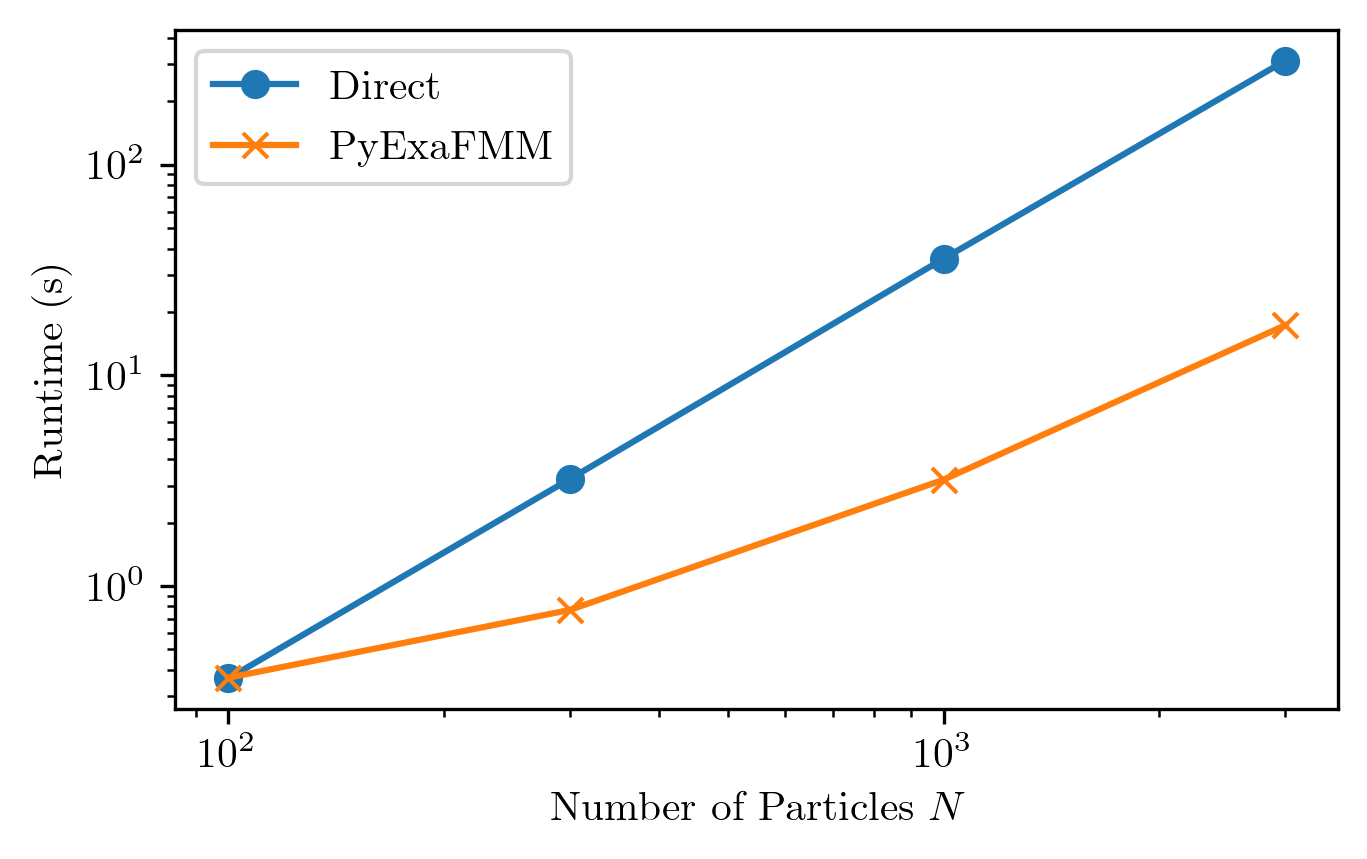
\includegraphics[width=0.8\textwidth]{assets/complexity.png}
    \end{figure}
\end{frame}

\begin{frame}{Outcomes - Optimum Target Rank Investigated}
    \begin{figure}
        \centering
        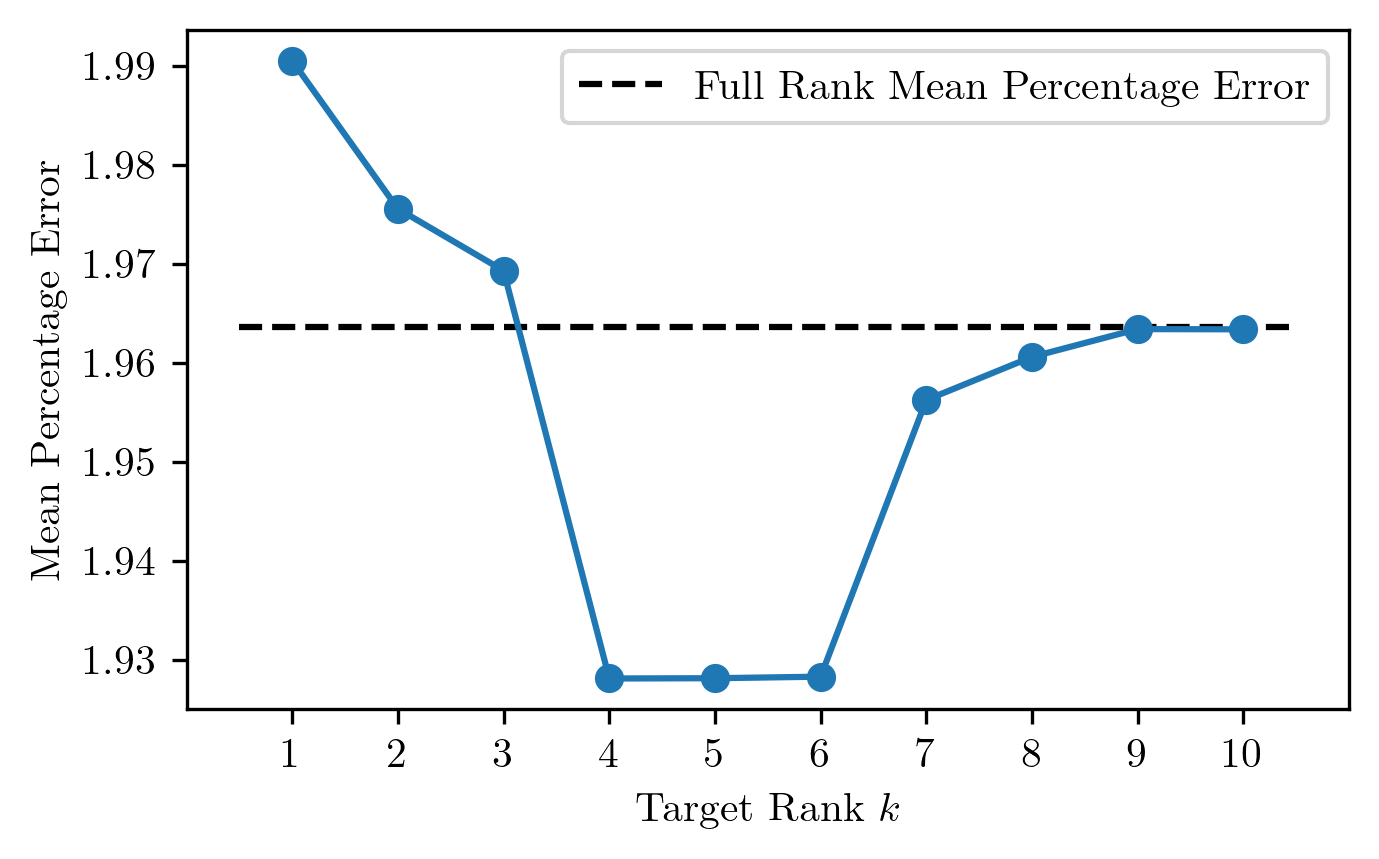
\includegraphics[width=0.8\textwidth]{assets/svd.png}
    \end{figure}
\end{frame}